\chapter{Test}
I udarbejdelsen af projektet har der været fokus på at teste systemet, så det hele tiden kunne verificeres at systemet havde den ønskede funktionalitet. I dette afsnit beskrives test af systemet, men for mere information omkring emnet henvises til dokumentationen\footnote{Se bilag - Dokmentationen, sektion 10}.
Systemet er blevet testet vha. unit test, continuous integration og manuelle tests.

\section{Unit tests}
Systemets unit tests er udarbejdet ved brug af NUnit \cite{NUnit} og NSubstitute \cite{NSubstitute}, som begge er test frameworks til .NET. Unittestene er skrevet i et separat projekt, så det ikke påvirkede selve BargainBarter projektet.
Generelt har unittestene den funktion, at verificere controllerne returnere de korrekte views, og kalder korrekt ned i eksempelvis databasen.
%Unittestene er generelt skrevet på controllers for at verificere, at disse returnerer de rigtige views og kalder rigtigt ned i f.eks. databasen eller ud i andre klasser. 
Tests i forbindelse med databasen er gjort muligt ved anvendelse af repository pattern. For en uddybende forklaring af dette henvises til dokumentationen \footnote{Se bilag - Dokumentation, sektion 9.8}.

\section{Manuelle tests}
Det valgte design af applikationen har betydet, at det ikke har været muligt at automatisere alle tests. Grundet dette har de automatiserede tests været suppleret meget med manuelle tests. Dette er foregået ved at en bruger har klikket rundt på hjemmesiden, og bekræftet om den nyimplementerede funktionalitet virkede. Dette har eksempelvis været tilfældet ved bytteflowet, som kan ses på figur \ref{fig:bytteflow}. 
Her er det Konkret gjort ved at en bruger er gået igennem dette flow og be- eller afkræftet om dette virkede efter hensigten.
%Dette er gjort ved at en bruger har klikket igennem dette flow og be- eller afkræftet om dette virker efter hensigten.

\begin{figure}[H]
	\centering
	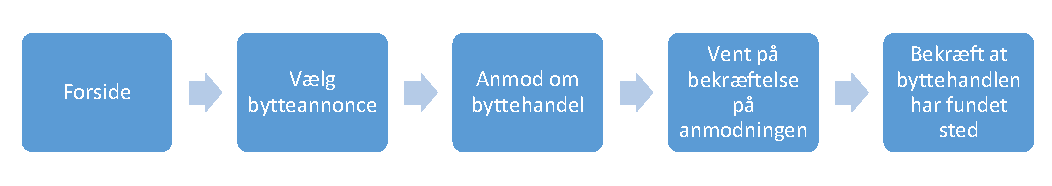
\includegraphics
	[width=140mm]{figures/bytteflow.pdf}
	\caption{Flow over en byttehandel i BargainBarter}
	\label{fig:bytteflow}
\end{figure}

\section{Test erfaringer}
\noindent Det har vist sig at controllers der benytter HTTP specifikke metoder/information, har været svære at teste via automatiserede tests. Der er derfor blevet lavet manuelle tests i stedet. Da en stor del af projektets controllerer, har benyttet sig er HTTP metoder, ville det derfor have været prisværdigt at kunne automatisere de dertilhørende tests. Dette kunne i projektet have været opnået ved at adskille forretningslogikken fra controllers. På denne måde ville controllers udelukkende stå for interaktionen mellem views og database, og udover dette uddelegerer forretningsspecifikke handlinger til separate klasser. En illustration af dette kan ses på figur \ref{fig:businesslogik}.

\begin{figure}[H]
	\centering
	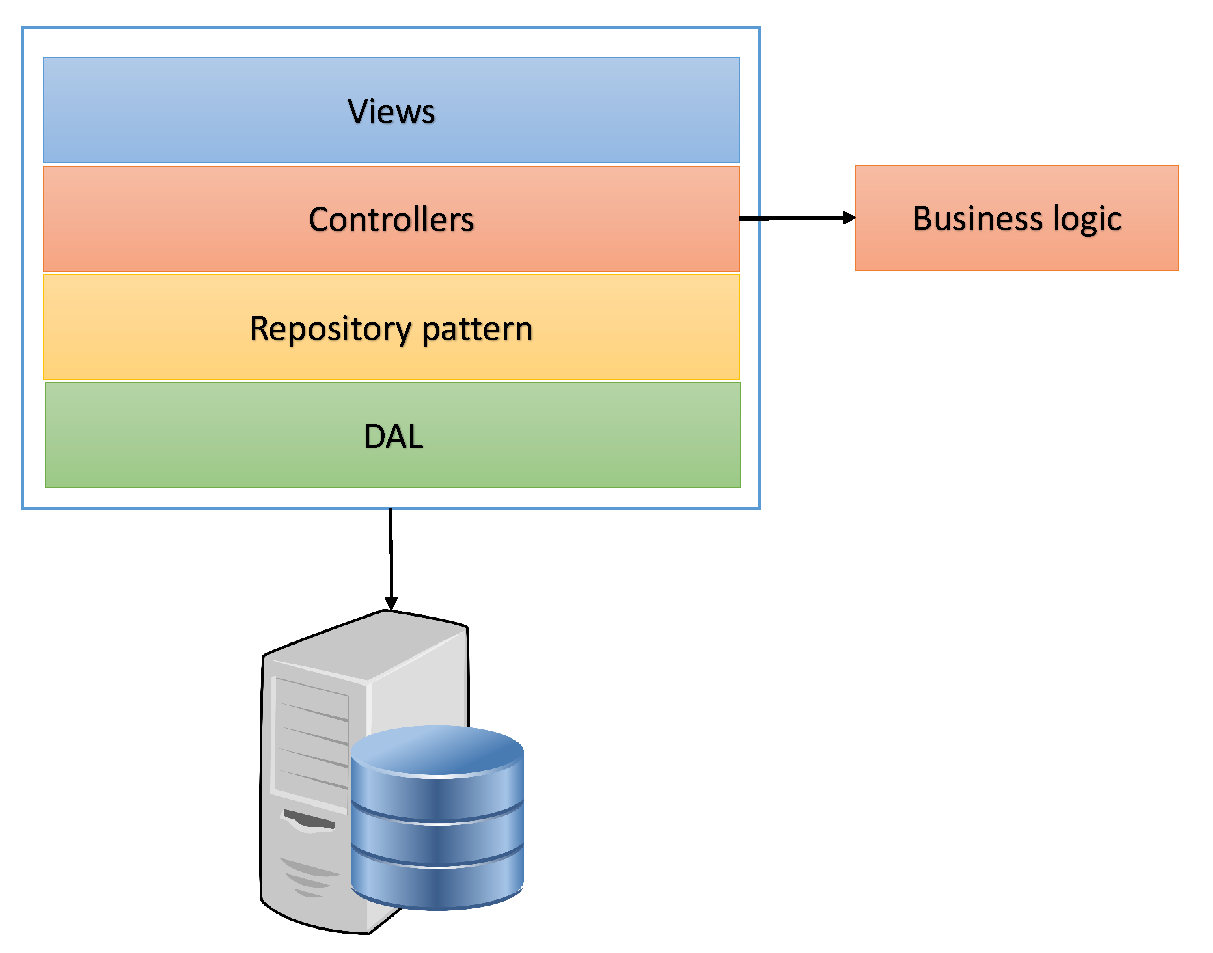
\includegraphics
	[width=140mm]{figures/businesslogik.pdf}
	\caption{Illustration af udvidet design til BargainBarter}
	\label{fig:businesslogik}
\end{figure}

Denne klasses forretningslogik  ville på denne måde lettere kunne testes.

\section{Continuous integration}
Continuous integration blev sat op ved brug af TeamCity \cite{TeamCity}. TeamCity-serveren blev sat op til at overvåge gruppens github-repository, så hvert push til repositoriet medførte et build på TeamCity serveren. På TeamCity var to builds sat op i en pipeline. Det første build byggede projektet. Hvis det første build lykkedes, blev det andet build kørt. Dette build kørte alle de tilhørende test til projektet ved brug af et indbygget NUnit-plugin i TeamCity. På baggrund af disse test genererer TeamCity en rapport, der indeholder resultatet af de kørte test, samt en coverage-analyse, der belyste, hvor stor en del af koden testene dækkede\footnote{Se bilag for TeamCity rapporten}. \\ \\

% Igennem disse redskaber har gruppen opnået erfaringer om hvordan man laver et testbart design.
